\documentclass[a4paper]{scrartcl}
\usepackage{amsmath,amssymb,amsthm}
\usepackage{bm}
\usepackage{biblatex}
\usepackage{float}
\usepackage[colorlinks=true, allcolors = black, urlcolor=cyan]{hyperref}
\usepackage{graphicx}
\usepackage{listings}
\usepackage{mathtools}
\usepackage{matlab-prettifier}
\usepackage{physics}
\usepackage{verbatim}

\renewcommand{\thesection}{\arabic{section}}
\renewcommand{\thesubsection}{\alph{subsection}}

\title{Assignment 4}
\subtitle{TTK4210 - Advanced Control of Industrial Processes}
\author{Sondre Myrberg}
\date{\today}

\setlength{\parindent}{0pt} % Disable indentation
\mathtoolsset{showonlyrefs} % Only show equation numbers on referenced equations


\begin{document}

\hypersetup{pageanchor=false}
\begin{titlepage}
    \maketitle
    \vfill
    \vfill
    \vfill
    \vfill
    \vfill
    
\includegraphics[width=0.95\textwidth]{../ntnu_logo.pdf}
    \vfill
    \vfill
\end{titlepage}
\hypersetup{pageanchor=true}

\section{}
Considering the system

\begin{equation}\label{eq:1system}
	G(s) = \begin{bmatrix}
		\frac{3(s+2)}{(s+3)(s+1)} & \frac{2}{s+1} \\
		\frac{1}{s+2} & \frac{1}{s+3}
	\end{bmatrix}
\end{equation}

\subsection{}
The poles of the system can by Theorem 4.4 in the book be found by observing $\phi(s)$. This corresponds to the least common denominator of all non-identically zero minors of all orders of $G(s)$. By looking at \eqref{eq:1system} we have four minors of order 1, the elements of $G(s)$, and one minor of order 2, which is $\det{G(s)}$. This yields

\begin{equation}
	\begin{aligned}
		\det{G(s)} &= \frac{3(s+2)}{(s+3)^2(s+1)} - \frac{2}{(s+2)(s+1)} = \frac{3(s+2)^2 - 2(s+3)^2}{(s+3)^2(s+2)(s+1)}\\
		&= \frac{s^2-6}{(s+3)^2(s+2)(s+1)}
	\end{aligned}
\end{equation}
We then easily see that
\begin{equation}
	\begin{aligned}
		\phi(s) &= (s+3)^2(s+2)(s+1)
	\end{aligned}
\end{equation}
and we have two poles at $s=-3$, one pole at $s=-2$ and one pole at $s=-1$.\\
The zeros of the system can by Theorem 4.5 in the book be found by looking at the greatest common divisor of all the numerators of all order-r minors of $G(s)$, where r is the normal rank of $G(s)$. In this case we have that r is 2, hence we must look at the second order minor $\det{G(s)}$. This gives us that the zeros of $\det{G(s)} = \frac{\prod_i(s-z_i)}{\phi(s)}$ are also the zeros of the system. In our case this gives us zeros at $s = \pm \sqrt{6}$, and we have one RHP-zero at $s=\sqrt{6}$.

\subsection{}
The pole vectors of a system is given by
\begin{equation}
	\begin{aligned}
		u_{p_i} &\triangleq B^H q_i\\
		y_{p_i} &\triangleq C t_i
	\end{aligned}
\end{equation}
for respectively input pole vecor and output pole vector corresponding to the i'th pole and corresponding eigenvector. By using the code shown in \autoref{lst:polevec}
\begin{lstlisting}[style=Matlab-editor, caption=Matlab code to generate pole vectors, label={lst:polevec}]
g11 = tf([3 6],[1 4 3]); g12 = tf(2,[1 1]);
g21 = tf(1, [1 2]);      g22 = tf(1, [1 3]);
G = [g11 g12 ; g21 g22];

sys_ss = ss(G);
A = sys_ss.A; B = sys_ss.B; C = sys_ss.C; D = sys_ss.D;

[T, Po] = eig(A);
yp = C*T;
[Q, Pi] = eig(A');
up = B'*Q;
\end{lstlisting}
we get the output
{\small \begin{verbatim}
	up =

   -1.7889   -1.1094    1.0000         0         0
         0         0         0    2.0000    1.0000

    yp =

   -0.4160   -0.6708         0    1.0000         0
         0         0    1.0000         0    1.0000
\end{verbatim}
}
which is the input and output pole vectors of the system. The pole directions are given as the normalized pole vectors, which in this case is trivial to compute as all pole vectors have only one non-zero entry. \\
By Theorem 4.1 we have that a system is controllable if and only if every pole $p_i$ is controllable, and the pole $p_i$ is controllable if and only if
\begin{equation}
	u_{p_i} = B^H q_i \neq 0
\end{equation}
From above we see that all columns of \texttt{up} are non-zero, hence the system is controllable. Similarly for observability we have by Theorem 4.2 that a system is observable if and only if every mode $p_i$ is observable, and the mode $p_i$ is observable if and only if 
\begin{equation}
	y_{p_i} = Ct_i \neq 0
\end{equation}
As above we see that all columns of \texttt{yp} are non-zero, and our system is observable.

\subsection{}
The relative gain array of a system is given as
\begin{equation}
	\begin{aligned}
		\text{RGA}(G) &= \Lambda(G) \triangleq G \cross (G^{-1})^\top
	\end{aligned}
\end{equation}
where $\cross$ denotes the element wise multiplication of the matrices $G$ and $(G^{-1})^\top$. We here use the steady-state gain matrix $G(0)$ and compute the RGA-matrix with the MATLAB-code shown in \autoref{lst:RGA}.
\begin{lstlisting}[style = matlab-editor, caption = MATLAB code to generate the RGA-matrix, label = lst:RGA]
G_zero = evalfr(G,0);
RGA = G_zero.*inv(G_zero).';
\end{lstlisting}
This yields the RGA-matrix
{\small \begin{verbatim}
	RGA =

   -2.0000    3.0000
    3.0000   -2.0000
\end{verbatim}
}
By observing this and looking at the pairing rules given in the book, we want pairings with elements close to one, but more important we want to avoid pairing with negative elements. The natural choice of pairing is then $y_1$ with $u_2$ and $y_2$ with $u_1$. This is implemented as shown in \autoref{fig:sys_diag_pair}. The controllers are here both simple PI-controllers with $K_p = 1$ and $T_i = 1$. The output responses of the system with these controllers with unit steps in both references at different times are shown in \autoref{fig:resp_diagonal}.

\begin{figure}[ht!]
	\centering
	\includegraphics[width=0.8\textwidth]{fig/sys_diag_pair.pdf}
	\caption{System with diagonal pairing}
	\label{fig:sys_diag_pair}
\end{figure}
\begin{figure}[ht!]
	\centering
	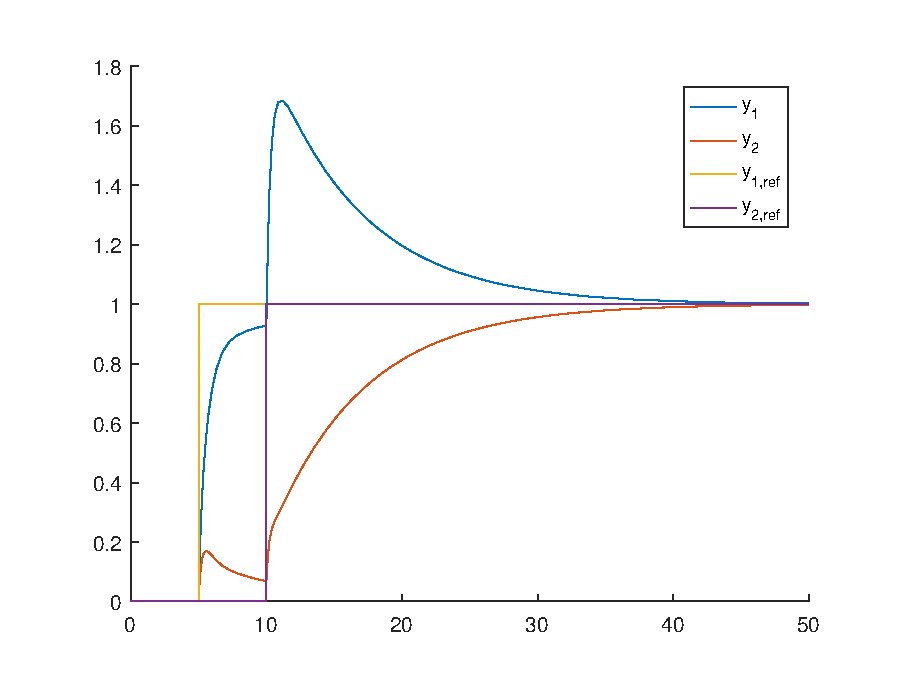
\includegraphics[width=0.8\textwidth]{fig/resp_diagonalpairing_stable.eps}
	\caption{Response with diagonal pairing and steps in references}
	\label{fig:resp_diagonal}
\end{figure}

%\clearpage

\subsection{}
Using the opposite pairing we get an unstable system as shown in \autoref{fig:resp_opposite_unstable}. This can however be counteracted by having negative gain in one of the controllers. Setting $K_{p,1} = -0.1$ we get the response shown in \autoref{fig:resp_opposite_stable}. This yields a stable plant, but is not a desirable solution as at once you take one of the loops out of service the whole plant becomes unstable.
\begin{figure}[ht!]
	\centering
	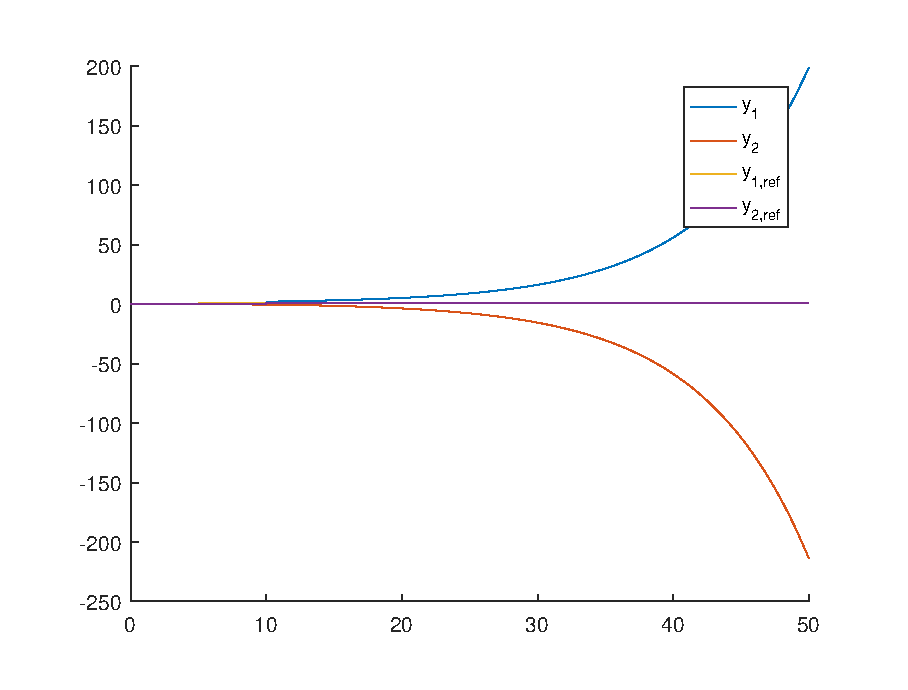
\includegraphics[width=0.8\textwidth]{fig/resp_oppositepairing_unstable.eps}
	\caption{Response of system with the opposite pairing}
	\label{fig:resp_opposite_unstable}
\end{figure}

\begin{figure}[ht!]
	\centering
	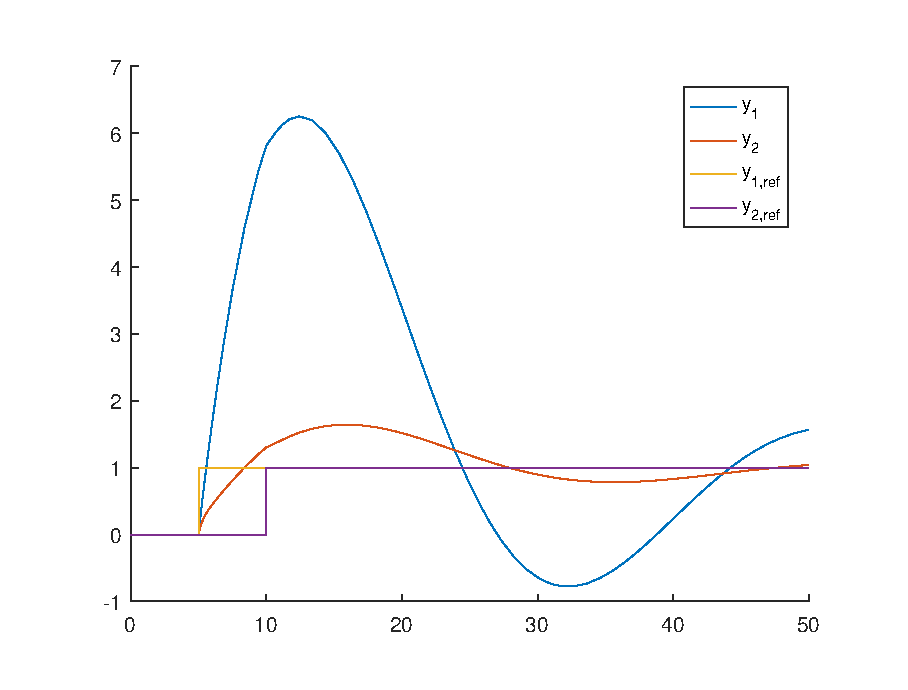
\includegraphics[width=0.8\textwidth]{fig/resp_oppositepairing_stable.eps}
	\caption{Response of system with opposite pairing and negative gain}
	\label{fig:resp_opposite_stable}
\end{figure}

\end{document}

